\documentclass[11pt]{article}
\usepackage[a4paper,margin=2.5cm]{geometry}
\usepackage{amsmath,amssymb}
\usepackage{graphicx}
\usepackage{hyperref}
\usepackage{booktabs}
\usepackage{enumitem}
\usepackage{xcolor}
\usepackage{caption}

\hypersetup{colorlinks=true, linkcolor=blue, urlcolor=blue, citecolor=blue}

\newcommand{\note}[1]{\par\noindent\fcolorbox{gray}{gray!8}{\parbox{0.96\textwidth}{\small\textbf{Implementation note.} #1}}\par\vspace{4pt}}

\title{\Large Visual-Inertial Odometry (VIO)\\[2pt]\large Robotic Systems 1 --- Course Project}
\author{Panagiotis Kiousis \and Stefanos Fotopoulos}
\date{English, extended version of the original report (9 June 2025)}

\begin{document}
\maketitle

\begin{center}
\small\textit{This is an extended English version of the original Greek report for this project. All
original content is included; a few derivations and discussion points have been added for clarity
and are marked as such. The original Greek report remains available in the repository
(\texttt{project/ERGASIA RS.pdf}) for reference.}
\end{center}

\section*{Introduction}
Visual-Inertial Odometry (VIO) estimates the trajectory of a moving camera by fusing data from a
stereo camera (Visual Odometry, VO) and an IMU. The two sources are combined with an Extended Kalman
Filter (EKF): the filter \emph{predicts} how the state evolves using a dynamics model driven by the
IMU, and then \emph{corrects} that prediction using an external observation (here, the VO estimate).

Within this fusion, we chose to work, at every time step, with the \emph{relative} transformation
between consecutive frames, for both the inertial and the visual branch, rather than with absolute
poses. These relative transformations are the inputs (both the control input $u$ and the measurement
$z$) to the EKF. This choice ensures that the correction step of the EKF has a substantial, direct
effect on the state estimate at every step, rather than being washed out by an ever-growing absolute
pose.

The dataset used is one of the sequences of the TUM Visual-Inertial Dataset
(\texttt{dataset-corridor4\_512\_16}). It contains stereo video from the two cameras of the data
collection rig (``corridor4''), IMU recordings, the relative poses between the sensors, sensor
calibration errors, and calibration information. Before reaching the core of the pipeline, some
preprocessing of the raw data was necessary.

\section{Inertial Odometry}

\subsection{Preprocessing the inertial data}
The IMU (Inertial Measurement Unit) measures quantities related to the motion and orientation of a
rigid body. In this dataset, at every time instant the IMU records a vector
$u = [\omega_x,\omega_y,\omega_z,a_x,a_y,a_z]^T \in \mathbb{R}^6$: angular velocity in 3 axes (rad/s)
and linear acceleration in 3 axes (m/s$^2$), both expressed in the IMU's body frame.

The cameras sample at 20 Hz (20 fps), while the IMU samples at 200 Hz. The IMU data therefore had to
be downsampled to match the camera rate. Simply keeping 1 measurement out of every 10 would discard
9 out of 10 samples and increase the noise of the kept sample; instead, every block of 10 consecutive
measurements is averaged, producing the downsampled sequence used as the EKF's prediction-step input
(implemented in \texttt{downsample\_inertial.py}).

\subsection{State modeling}
The state vector consists of position, orientation (as Euler angles) and velocity in the world frame:
\[
m = [x,y,z,\phi,\theta,\psi,v_x,v_y,v_z]^T, \qquad (x,y,z) \text{ position}, \quad (\phi,\theta,\psi)
\text{ Euler angles}, \quad (v_x,v_y,v_z) \text{ velocity}.
\]

\subsection{System dynamics model (prediction step)}
The dynamics are based on integrating the IMU measurements and are implemented in
\texttt{imu\_dynamics(mu, u, dt=0.05)}, which takes the current state \texttt{mu} and the IMU input
\texttt{u}. The function reads the position, orientation (as Euler angles) and velocity from \texttt{mu}.
From the input \texttt{u}, it takes the angular velocity and linear acceleration in the body frame.
The orientation is updated with a simple Euler integration: the angular velocity is first rotated into
the world frame and then integrated over $dt$. The accelerations are then rotated from the body frame
into the world frame, and gravity is subtracted. The resulting world-frame acceleration updates the
velocity and finally the position. The result is the predicted state after a time step $dt$:
\begin{align}
R_{\text{world}} &= \texttt{euler\_to\_rot}(\text{orientation})\\
\omega_{\text{world}} &= R_{\text{world}} \cdot \omega_{\text{body}}\\
\text{orientation}_{\text{new}} &= \text{orientation} + \omega_{\text{world}} \cdot \Delta t\\
R_{\text{world}} &= \texttt{euler\_to\_rot}(\text{orientation}_{\text{new}})\\
a_{\text{world}} &= R_{\text{world}} \cdot a_{\text{body}} - g\\
v_{\text{new}} &= v + a_{\text{world}} \cdot \Delta t\\
p_{\text{new}} &= p + v_{\text{new}} \cdot \Delta t + \tfrac{1}{2} a_{\text{world}} \cdot (\Delta t)^2
\end{align}
where $\omega_{\text{body}}$ and $a_{\text{body}}$ are the IMU's angular velocity and acceleration,
$g = [0,0,9.81]^T$ is gravitational acceleration, and $dt = 0.05\,\mathrm{s}$ (camera rate 20 Hz, IMU
rate 200 Hz, downsampled to 20 Hz).

\subsection{Jacobian of the dynamics model}
The function \texttt{imu\_jacobian} computes the Jacobian of the dynamics function with respect to the
state \texttt{mu}, using a numerical approximation via finite differences. The Jacobian matrix
expresses how small perturbations in the current state affect the predicted next state, and is
essential to algorithms such as the Extended Kalman Filter. The function first computes the nominal
evolution $f(\mu)$; then, for each state component, it applies a small perturbation $\epsilon$,
recomputes the dynamics, and approximates the derivative as a difference quotient. Column $i$ of the
matrix contains the effect of perturbing state variable $i$ on the entire output, so the result is the
Jacobian matrix:
\[
F = \frac{\partial f}{\partial \mu} \approx \frac{f(\mu+\epsilon)-f(\mu)}{\epsilon}.
\]

\note{Why finite differences rather than an analytic Jacobian. The dynamics function composes two
rotations that both depend on the orientation state (one to rotate $\omega_{\text{body}}$ into the
world frame using the \emph{old} orientation, one to rotate $a_{\text{body}}$ using the \emph{updated}
orientation), so the analytic Jacobian is not block-diagonal: a perturbation of any Euler angle
propagates into the acceleration, velocity \emph{and} position rows. Qualitatively, with the state
ordered as (position, orientation, velocity), $F$ has the following block sparsity structure (rows =
output blocks, columns = blocks differentiated with respect to):
\[
F =
\begin{bmatrix}
I & \dfrac{\partial p_{\text{new}}}{\partial \text{ori}} & \Delta t\, I \\[4pt]
0 & I + \Delta t\,\dfrac{\partial \omega_{\text{world}}}{\partial \text{ori}} & 0 \\[4pt]
0 & \dfrac{\partial a_{\text{world}}}{\partial \text{ori}} \Delta t & I
\end{bmatrix}
\begin{array}{l}\leftarrow \text{pos}\\ \leftarrow \text{ori}\\ \leftarrow \text{vel}\end{array}
\]
(columns, left to right: pos, ori, vel). The only genuinely nontrivial blocks are the derivatives of
$\omega_{\text{world}} = R_{\text{world}}
\omega_{\text{body}}$ and $a_{\text{world}} = R_{\text{world}} a_{\text{body}}$ with respect to the
Euler angles — each is a derivative of a rotation matrix acting on a fixed body-frame vector, i.e. a
sum of terms of the form $\frac{\partial R}{\partial \phi}\,v$, $\frac{\partial R}{\partial
\theta}\,v$, $\frac{\partial R}{\partial \psi}\,v$, each a $3\times 3\to 3$ linear map obtained by
differentiating the Euler-angle rotation matrix. Deriving and maintaining this symbolically for an
$xyz$-Euler parametrization is error-prone and gains little in practice at a 20 Hz update rate with
$\epsilon = 10^{-5}$, so central-difference-free forward finite differences (as implemented) is a
reasonable, robust engineering choice; it costs $O(n)$ extra evaluations of $f$ per Jacobian ($n=9$
here), which is negligible at this problem size.}

\section{Visual Odometry}
The EKF's correction step uses as measurement $z_t$ the homogeneous transformation produced by visual
odometry. How is that transformation obtained? The dataset provides, among other things, the camera
frames for each camera separately and the calibration data. The pipeline processes the frames,
finds features in them, matches features both between the two cameras and across time, and finally
produces 3D point clouds and the homogeneous transformations between consecutive frames. Each step is
analyzed separately below.

\subsection{Undistortion}
Because of lens curvature, a camera's rays are distorted, so the captured photo/frame does not match
the real-world image. From the dataset we are given the type of camera distortion (radial) and its
model. For a point at radius $r$ from the image center, $r^2 = x^2+y^2$, the radial distortion model
is
\[
x_{\text{distortion}} = x_d = x(1+k_1 r^2+k_2 r^4), \qquad
y_{\text{distortion}} = y_d = y(1+k_1 r^2+k_2 r^4),
\]
with the coefficients $k_i$ given in \texttt{camchain.yaml} (variable \texttt{distortion\_coeffs}). In
addition to radial distortion, the cameras also exhibit tangential distortion, caused by imperfect
sensor/lens alignment, which often produces inaccuracies toward the edges of the image. That model is
\[
x_d = x + [2p_1 xy + p_2(r^2+2x^2)], \qquad y_d = y + [p_1(r^2+2y^2)+2p_2 xy],
\]
with the coefficients $p_i$ from the same file and variable. Removing these distortions requires
inverting these relations for $x,y$, which is difficult in closed form because $r$ appears nonlinearly
(through its square) on both sides. We therefore use the \texttt{cv2} library to perform this
nonlinear inversion: the library solves the problem numerically and approximates the true solution
with very small error, via Newton's method, returning the undistorted $(x,y)$ pairs.

\note{What the code actually uses. \texttt{step1 undistortion.py} calls
\texttt{cv2.fisheye.undistortImage}, i.e. OpenCV's \emph{equidistant} fisheye model
($r_d = r\,(1+k_1 r^2+k_2 r^4+k_3 r^6+k_4 r^8)$ on the angle-derived radius $r$, not the classical
radial/tangential model written above), consistent with the TUM-VI rig's wide-FOV lenses. The
radial+tangential equations above are the general pinhole-distortion model described in the original
report and are kept here for completeness; in this project they describe the type of distortion
conceptually, while the actual numerical correction is carried out by OpenCV's fisheye routine with
the dataset's $(k_1,k_2,k_3,k_4)$ fisheye coefficients, not by manually inverting the two equations
above. No tangential term is used in the code, since the equidistant fisheye model does not include
one.}

\subsection{Rectification}
The next issue is that we have a stereo camera system, so we need to reconcile the information from
the two cameras in a way that is useful later for depth computation per frame.

To do this, we start from epipolar geometry, which defines the epipolar planes formed by 3D points and
the optical centers of the two cameras (3 points total that determine a plane in space). It also
defines the epipolar lines, which are the intersections of those planes with the two cameras' image
planes. Each camera therefore sees the same point along a different line. If we rectify these two
cameras' epipolar lines, every point seen by one camera lies on the rectified epipolar lines of both
cameras, and corresponds to a point on those same lines in the other camera. So, if we only want to
search for points (for features we wish to track) in 3D, it suffices to search along the same epipolar
lines for both cameras (or within a small range of lines, to allow for error).

\begin{figure}[h]
  \centering
  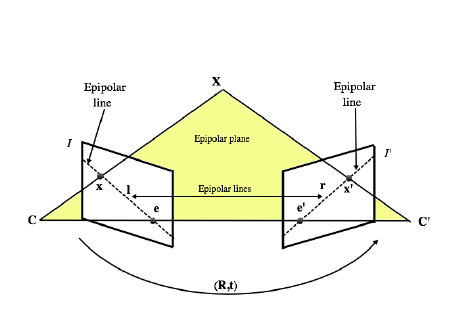
\includegraphics[width=0.6\textwidth]{figures/epipolar_geometry.png}
  \caption{Epipolar-line visualization (image used for illustration in the original report).}
\end{figure}

To do this we again use the \texttt{cv2} library, specifically the function \texttt{stereoRectify},
which performs this alignment. The procedure implemented by the function is as follows. It takes as
input the image size, the two cameras' intrinsic matrices, and the rotation and translation matrices
between the two cameras. The intrinsic matrices describe how 3D points are mapped onto the camera's 2D
image plane, and have the form
\[
K = \begin{bmatrix} f_x & 0 & c_x \\ 0 & f_y & c_y \\ 0 & 0 & 1 \end{bmatrix},
\]
where $f_x,f_y$ are the focal lengths of each camera and $c_x,c_y$ are each camera's principal point.
These matrices, as well as the homogeneous transformation between the two cameras containing the
rotation and translation, are stored in \texttt{camchain.yaml}.

With these known, new axes are constructed such that images are aligned with the $X$ axis parallel to
the line joining the two cameras' centers. Rotation matrices from the previous poses to these new axes
are then defined. In the new system, orientation is therefore identical, and the only thing that
changes between the new images, for the same point, is the position along the same epipolar line.

It is worth noting that after this process the two cameras have new intrinsic matrices, which in fact
coincide. The function returns the rotation matrices and the projection matrices (matrices that show
the 2D projection from a given 3D position and orientation of each camera):
\[
P_1 = K_{\text{new}}\begin{bmatrix} I & 0 \end{bmatrix}, \qquad
P_2 = K_{\text{new}}\begin{bmatrix} I & T_{\text{new}} \end{bmatrix}, \quad T_{\text{new}}=[\Delta x,0,0]^T.
\]
The rectified, distortion-free images are then generated and stored.

\subsection{Feature detection}
Once the images are prepared, we move to the basic building blocks of visual odometry. To estimate
motion, we need to find features in each frame that we can track across frames to compute the system's
motion. For this we chose between algorithms such as FAST and SIFT. The former is faster, but since
this is offline VIO, we chose the latter, which gives better results. Besides finding features, SIFT
also computes a descriptor for each feature, i.e. a unique identifier based on the region around it, so
that the same feature can be tracked over time without confusing it with others.

\textbf{Keypoint detection.} The image/frame is progressively blurred with Gaussians of increasing
standard deviation $\sigma$, via convolution
\[
L(x,y,\sigma) = G(x,y,\sigma) * I(x,y),
\]
where $L$ is the new image, $G$ the Gaussian and $I$ the original image. As with the function $G$, we
apply filters that compute weighted sums over different regions, which blurs the original image at
different scales and, by comparing Gaussians at different scales, reveals detail at different
distances/scales. Every point that is a local maximum or minimum of these difference-of-Gaussian
responses is a candidate keypoint.

All candidate points are then used and the best ones are filtered, i.e. those with strong contrast
relative to neighboring points, avoiding edges as much as possible via a Hessian matrix that tests
curvature. A dominant orientation is also computed for each keypoint so that it can be described
consistently later.

Descriptors are then produced: vectors storing values that help identify features. They work by
encoding the neighborhood of the central pixel, taking into account the orientation mentioned above, by
rotating neighboring points to find which ones match/resemble it most closely. Normalization is also
used to make the matching more robust. This is how features are found and identified. Below is an
example visualization of feature detection in one image.

\begin{figure}[h]
  \centering
  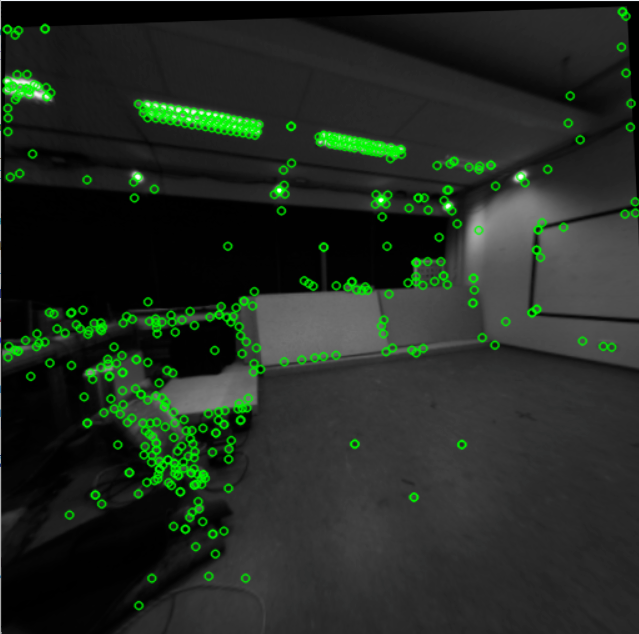
\includegraphics[width=0.55\textwidth]{figures/sift_keypoints.png}
  \caption{SIFT feature-detection visualization (detected keypoints overlaid on a rectified left-camera frame).}
\end{figure}

In code, SIFT is configured with \texttt{nfeatures=500}, \texttt{nOctaveLayers=3},
\texttt{contrastThreshold=0.02}, \texttt{edgeThreshold=15}, \texttt{sigma=1.6}.

\subsection{Feature matching}
Having identified the features and being able to distinguish them, the next step is to match the
features seen by each camera, and then the features seen by one camera over time.

\paragraph{Stereo matching.} Between the 2 cameras, we take in turn all the features of one camera, and
by searching all possible pairings (via a brute-force algorithm from \texttt{cv2}, \texttt{BFMatcher})
we find, via Euclidean distance
\[
D(d_1,d_2) = \sqrt{\sum_{i=1}^{128}(d_{1,i}-d_{2,i})^2},
\]
the 2 best matches in the second image for the feature. If the first match is substantially better than
the second, we are fairly confident it is the correct correspondence (Lowe's ratio test, threshold 0.75
in code). Since we also know, from rectification, that for rectified images the same feature will lie
on the same epipolar line, we add a filter that keeps only points on nearby epipolar lines (vertical
disparity below 2.0 pixels in code).

\paragraph{Temporal matching.} For temporal correspondences, we again use the brute-force matcher and
apply RANSAC filtering to keep only valid points. The algorithm performs many iterations of random
sampling of a few features, and at each iteration builds a candidate matrix $E$ encoding the rotation
and translation between the previous and next frame. After doing this many times, it selects the matrix
considered most representative, and for any points whose position in the previous and next frame is
not explained by that matrix, they are treated as outliers and removed from the tracked features. The
relation giving the matrix $E$, and the one that is checked to decide whether points belong to the
inlier set, is
\[
E = [t]_\times R, \qquad p_{t+1}^T E\, p_t = 0.
\]
In code this is \texttt{cv2.findEssentialMat} with \texttt{method=cv2.RANSAC}, confidence $0.999$,
reprojection threshold $1.0$ pixel.

This gives a robust way to track features both in space and in time. A visualization of this step
follows.

\begin{figure}[h]
  \centering
  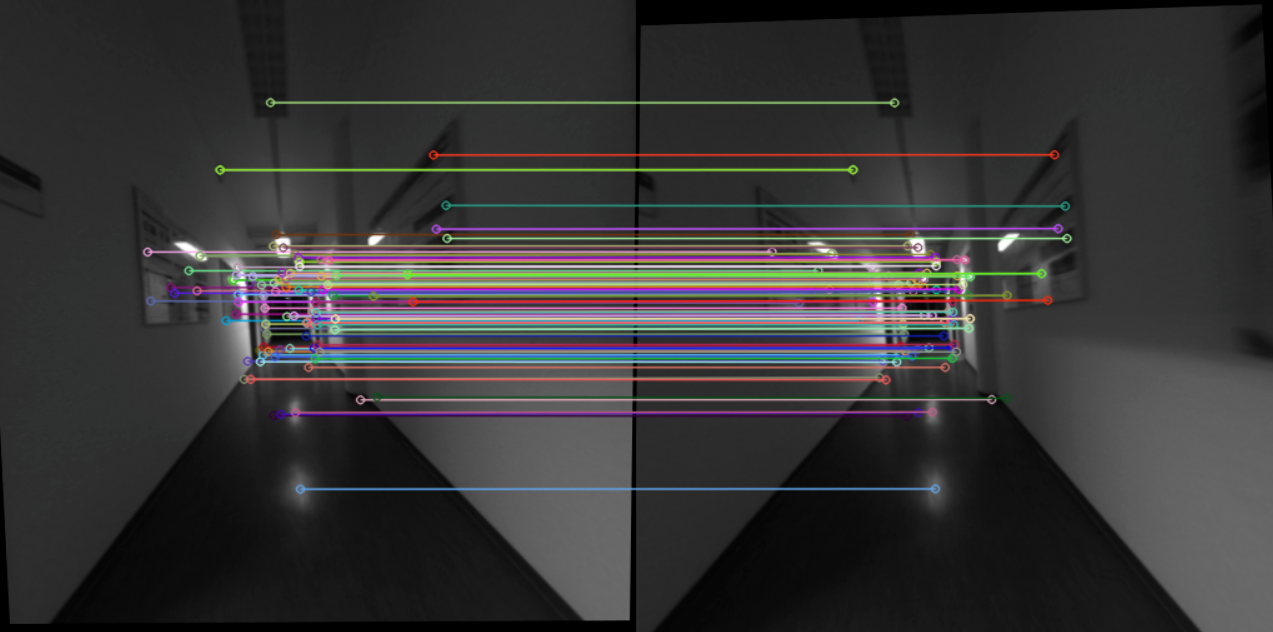
\includegraphics[width=0.85\textwidth]{figures/temporal_matching.png}
  \caption{Feature matching between the two cameras (stereo matches, shown as connecting lines between the left and right frame).}
\end{figure}

\subsection{Point cloud}
To compute the transformations describing motion between frames, we decided to use a 3D point cloud
tracked over time, which gives a good estimate of the system's rotation and translation.

The relations used to compute the coordinates, and especially the depth, of each feature are
\[
Z = \frac{fB}{d}, \qquad X = \frac{Z(u_{\text{left}}-c_x)}{f}, \qquad Y = \frac{Z(v_{\text{left}}-c_y)}{f},
\]
where $f$ is the (shared) focal length of the two cameras, $B$ is the baseline between the two
cameras' centers, and $d$ is the horizontal disparity ($d = u_{\text{left}} - u_{\text{right}}$).

\note{What the code actually uses. Rather than coding these classical stereo-triangulation relations
directly — which would be slower, less numerically robust, and biased for near-degenerate
configurations — \texttt{step4 pointcloud.py} uses \texttt{cv2.triangulatePoints}, OpenCV's linear DLT
triangulation from the two projection matrices $P_1,P_2$ (from rectification) and the matched 2D
points. This is mathematically equivalent to the disparity formulas above for a rectified stereo pair,
but is more numerically robust and directly consistent with $P_1,P_2$ as actually computed by
\texttt{stereoRectify}. The code additionally filters out points with depth outside $[0.1,50]\,\mathrm{m}$
before keeping them for the next stage.}

Below we see an example of the resulting 3D cloud, shown rotated, with depth encoded by color
(cooler colors farther away). The trajectory along the corridor is clearly visible.

\begin{figure}[h]
  \centering
  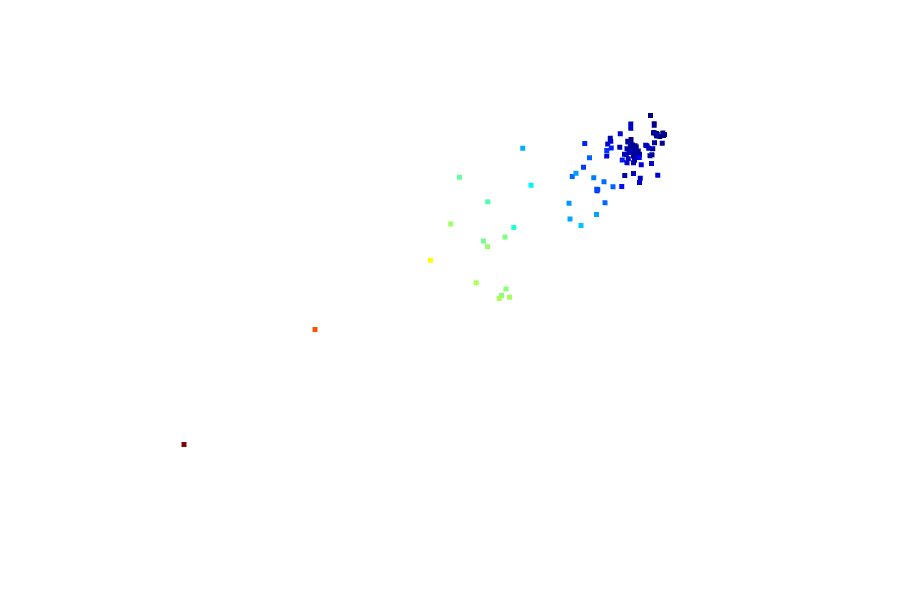
\includegraphics[width=0.55\textwidth]{figures/pointcloud_3d.png}
  \caption{3D point-cloud visualization.}
\end{figure}

\subsection{Trajectories}
Next is the estimation of the homogeneous transformation between each point cloud and its predecessor.
For this we use the Kabsch algorithm, which computes the best-fit rotation and translation between two
point sets. Specifically, we first compute the means of the $N$ matched points in each dimension, both
for the previous and the next cloud:
\[
p_p = \begin{bmatrix}x_p\\y_p\\z_p\end{bmatrix}, \quad
\bar p_p = \frac1N\sum_{i=1}^N p_p =
\begin{bmatrix}\frac1N\sum_i x_p\\ \frac1N\sum_i y_p\\ \frac1N\sum_i z_p\end{bmatrix},
\qquad
p_n = \begin{bmatrix}x_n\\y_n\\z_n\end{bmatrix}, \quad
\bar p_n = \frac1N\sum_{i=1}^N p_n =
\begin{bmatrix}\frac1N\sum_i x_n\\ \frac1N\sum_i y_n\\ \frac1N\sum_i z_n\end{bmatrix}.
\]
We then subtract the mean from every point and compute a cross-covariance matrix $H$:
\[
H = \sum_{i=1}^N (p_{n_i}-\bar p_n)(p_{s_i}-\bar p_s)^T,
\]
whose singular value decomposition (SVD) yields the rotation matrix
\[
R = VU^T
\]
(with a reflection correction when $\det R < 0$, applied in code but omitted from the original report),
which is the best-fit rotation between the two sets. The translation is then
\[
t = \bar p_n - R\bar p_s.
\]
This gives the homogeneous transform from each frame to the next:
\[
T = \begin{bmatrix} R_{3\times 3} & t_{3\times 1} \\ 0 & 1 \end{bmatrix}.
\]
Chaining all frames together gives the estimated odometry/trajectory shown below. Before that,
however, it is worth analyzing the covariance matrix computed at this step, since it essentially
expresses the confidence in the correctness of the odometry estimate. This works as follows. First, the
estimate from the previous cloud for the next one is computed as
\[
\hat p_t = R p_s + t,
\]
and the error from the actual position of the cloud in the next state is then computed. A variance
$\sigma^2$ is estimated from the mean squared residual, which, combined with the Jacobian for each pair
of points, yields the covariance matrix
\[
Q = \sigma^2\Big(\sum_{i=1}^N J_i^T J_i\Big)^{-1},
\]
which measures the uncertainty of the measurement and is used for this purpose in the Kalman filter as
the EKF's measurement noise. The visual-odometry results are:

\begin{figure}[h]
  \centering
  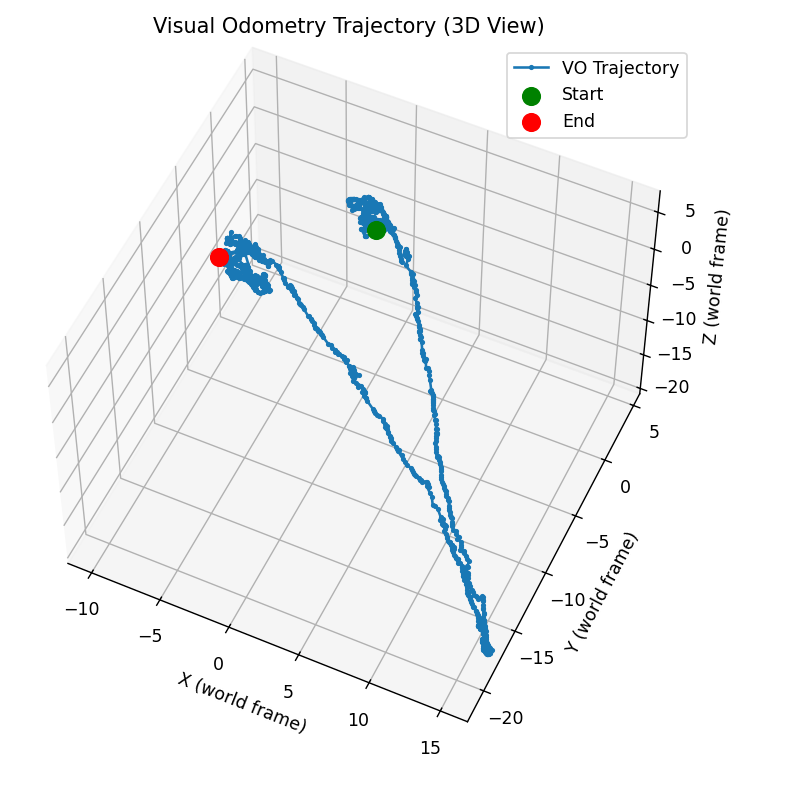
\includegraphics[width=0.7\textwidth]{figures/vo_traj_3d.png}
  \caption{Visual-odometry trajectory, 3D view.}
\end{figure}
\begin{figure}[h]
  \centering
  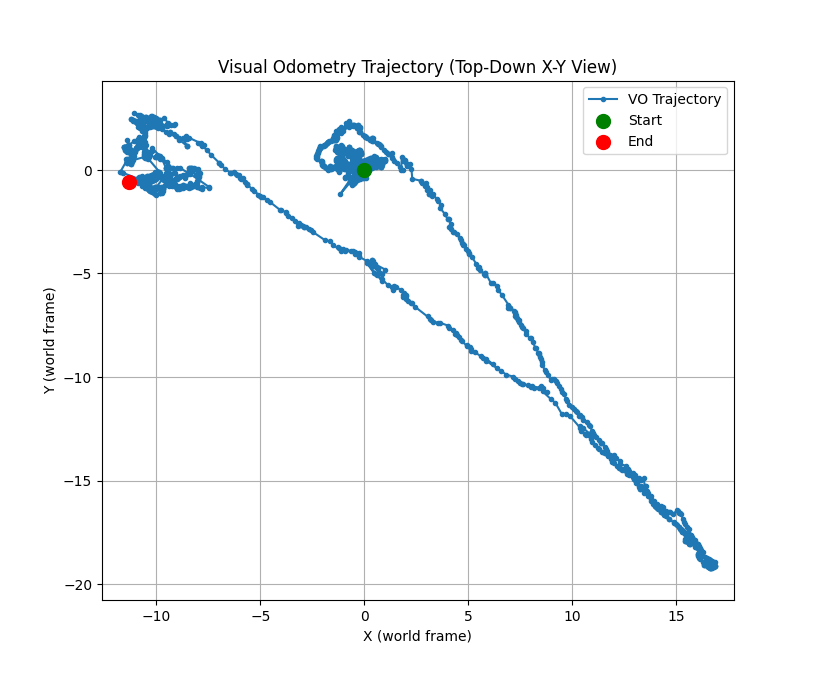
\includegraphics[width=0.7\textwidth]{figures/vo_traj_topdown.png}
  \caption{Visual-odometry trajectory, top-down X-Y view.}
\end{figure}

\note{What the code actually uses for $J_i$ and for $Q$ in the EKF. \texttt{step5 TVO.py} builds $J_i =
[-I_3 \;\; [R p_i]_\times]$ for each matched point pair (the Jacobian of the rigid-transform residual
with respect to the 6-DoF pose, position and rotation blocks), consistent with the formula above,
and falls back to a large covariance $\mathrm{diag}(10^3,\dots)$ when fewer than 6 point pairs are
available. However, in the final \texttt{ekf.py} the per-step VO covariance $Q_{cov,k}$ computed this
way is \emph{not} actually fed into the Kalman update — the line that would do so is commented out
(\texttt{\# Q\_cov\_k = qcov\_matrices[k]}), and a fixed $Q_{cov} = I_6\times 10^{-8}$ is used instead
for every step (Sec.~3.2). The per-step $Q$ above is therefore computed and saved, and is the
theoretically correct way to weight each VO measurement by its own uncertainty, but the EKF run that
produced the results in Sec.~4 used a constant $Q$. This is pointed out here for transparency and as a
natural improvement to revisit (feeding $Q_{cov,k}$ back into the EKF should make the filter trust
visually uncertain steps less, automatically, rather than through hand-tuning a single constant).}

\subsection{VO observation model}
The VO observation model returns a 6-vector of poses, with the position and orientation of the robot,
given by the transformation matrices: $h(\mu) = \mu[0{:}6] = [x,y,z,\phi,\theta,\psi]^T$. The Jacobian
of the observation describes how each element of the state affects each element of the observation.
The resulting matrix has size $6\times 9$ and contains the partial derivatives of each observation
component with respect to each input. Since both vectors contain position and orientation, this
produces a diagonal of ones, which is simply the derivative of each component with respect to itself.
The remaining entries are zero (for example, a small change in the $y$ input does not affect the $z$
observation). The result is
\[
H = \frac{\partial h}{\partial \mu} = [I_6,\, 0_{6\times 3}].
\]

\section{EKF Implementation}

\subsection{EKF uncertainty matrices}

\subsubsection{Constructing the uncertainty matrix $R_{\text{cov}}$}
IMU measurements are noisy. This noise introduces uncertainty into the state prediction. The matrix
$R_{\text{cov}} \in \mathbb{R}^{9\times 9}$ expresses how sensor noise (accelerometer, gyroscope)
propagates, through integration, into the state $m=[x,y,z,\phi,\theta,\psi,v_x,v_y,v_z]^T$. From
\texttt{imu\_config.yaml} we found the following IMU noise values:
\[
\sigma_a = \texttt{accel\_noise\_density} = 0.0028\ \mathrm{m/s^{1.5}} = \frac{\mathrm m}{\mathrm
s^2\sqrt{\mathrm{Hz}}}, \qquad
\sigma_\omega = \texttt{gyro\_noise\_density} = 0.00016\ \mathrm{rad/s^{0.5}} = \frac{\mathrm{rad}}{\mathrm
s\sqrt{\mathrm{Hz}}}.
\]
So, for each step $dt$:
\[
\mathrm{Var}(a) = \frac{\sigma_a^2}{dt}, \qquad \mathrm{Var}(\omega) = \frac{\sigma_\omega^2}{dt},
\]
and, depending on how many times the quantity is integrated to produce each state variable:
\[
\mathrm{Var}(\theta) = \mathrm{Var}(\omega)\cdot(dt)^2, \qquad
\mathrm{Var}(v) = \mathrm{Var}(a)\cdot(dt)^2, \qquad
\mathrm{Var}(p) = \mathrm{Var}(v)\cdot(dt)^2 = \mathrm{Var}(a)\cdot(dt)^4.
\]
So $R_{\text{cov}} = \mathrm{diag}\big(\mathrm{Var}(p),\mathrm{Var}(p),\mathrm{Var}(p),\mathrm{Var}(\theta),
\mathrm{Var}(\theta),\mathrm{Var}(\theta),\mathrm{Var}(v),\mathrm{Var}(v),\mathrm{Var}(v)\big)$.

\note{In the final run, this physically-derived $R_{\text{cov}}$ is overwritten in code by a flat
$R_{\text{cov}} = I_9 \times 10^{-4}$ right after being printed (\texttt{ekf.py}, line
\texttt{R\_cov = np.eye(9) * 1e-4}), so the results in Sec.~4 use this constant value, not the
noise-density-derived one above; the derivation is kept here because it documents the intended,
physically grounded construction and is a straightforward thing to re-enable.}

\subsubsection{Constructing the uncertainty matrix $Q_{\text{cov}}$}
The uncertainty matrix $Q$ is, in principle, obtained from the visual odometry according to the
analysis carried out above (Sec.~2.6) — see the implementation note there regarding what the final EKF
run actually used for $Q_{\text{cov}}$.

\subsection{EKF steps}
Below are the steps of the Extended Kalman Filter (EKF), used to estimate the state of a nonlinear
system by combining a model and an observation.

\subsubsection{State prediction (prediction step)}
In the first step, the future state is predicted based on the system dynamics and the input $u$.
\begin{itemize}[leftmargin=*]
  \item \textbf{State prediction:} $\bar\mu = f(\mu,u)$. The function $f$ predicts the new state of the
  system based on the motion model and the input $u$ (e.g. IMU data). In our case this is
  \texttt{imu\_dynamics}.
  \item \textbf{Covariance prediction:}
  \[
  F = \frac{\partial f}{\partial \mu}, \qquad \bar\sigma = F\cdot\sigma\cdot F^T + R.
  \]
  We compute the Jacobian $F$ of $f$ (via \texttt{imu\_jacobian}) and predict the uncertainty of the
  new state based on the current covariance $\sigma$ and the model uncertainty $R$.
\end{itemize}

\subsubsection{Correction with measurement (update step)}
\begin{itemize}[leftmargin=*]
  \item \textbf{Observation Jacobian:} $H = \dfrac{\partial h}{\partial \mu}$. $H$ describes how the
  state affects the measurement.
  \item \textbf{Kalman gain:} $K = \bar\sigma H^T(H\bar\sigma H^T+Q)^{-1}$. The Kalman gain $K$
  determines how much ``weight'' is given to the measurement $z$, relative to the predicted value,
  taking into account the uncertainties of both the prediction and the sensor.
  \item \textbf{State correction:} $\mu^+ = \bar\mu + K(z-h(\bar\mu))$. The new state estimate results
  from the predicted value and a correction via the difference between the actual and expected
  measurement.
  \item \textbf{Covariance update:} $\sigma^+ = (I-KH)\bar\sigma$. The new covariance reflects the
  reduced uncertainty after incorporating the measurement.
\end{itemize}

\subsubsection{Outputs}
\begin{itemize}[leftmargin=*]
  \item \texttt{mu\_new}: the final state estimate after prediction and correction.
  \item \texttt{sig\_new}: the updated uncertainty of the estimate.
\end{itemize}

\section{Results}
The trajectory produced by the EKF is smooth and incorporates both the dynamics and the VO
corrections, reducing errors caused by noise. Below are results for different values of the
uncertainty matrices $R$ and $Q$.

\subsection{Trusting prediction and observation equally}
\[
R_{\text{cov}} = I_9\times 10^{-4}, \qquad Q_{\text{cov}} = I_6\times 10^{-4}.
\]
\begin{figure}[h]
  \centering
  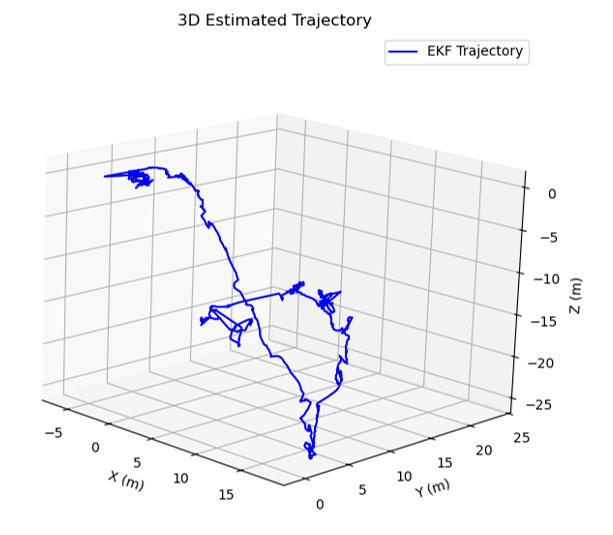
\includegraphics[width=0.6\textwidth]{figures/ekf_R1e-4_Q1e-4.png}
  \caption{EKF trajectory, $R_{\text{cov}}=10^{-4}I$, $Q_{\text{cov}}=10^{-4}I$.}
\end{figure}

\subsection{Trusting the inertial (prediction) branch more}
\[
R_{\text{cov}} = I_9\times 10^{-8}, \qquad Q_{\text{cov}} = I_6\times 10^{-4}.
\]
\begin{figure}[h]
  \centering
  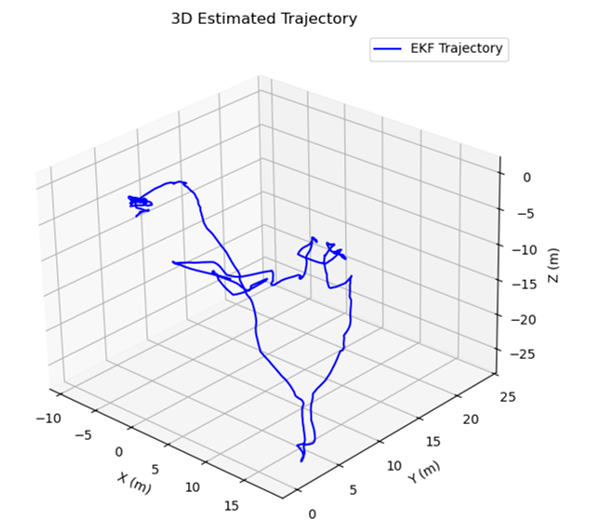
\includegraphics[width=0.6\textwidth]{figures/ekf_R1e-8_Q1e-4.png}
  \caption{EKF trajectory, $R_{\text{cov}}=10^{-8}I$, $Q_{\text{cov}}=10^{-4}I$.}
\end{figure}

\subsection{Trusting the visual (observation) branch more}
\[
R_{\text{cov}} = I_9\times 10^{-4}, \qquad Q_{\text{cov}} = I_6\times 10^{-8}.
\]
\begin{figure}[h]
  \centering
  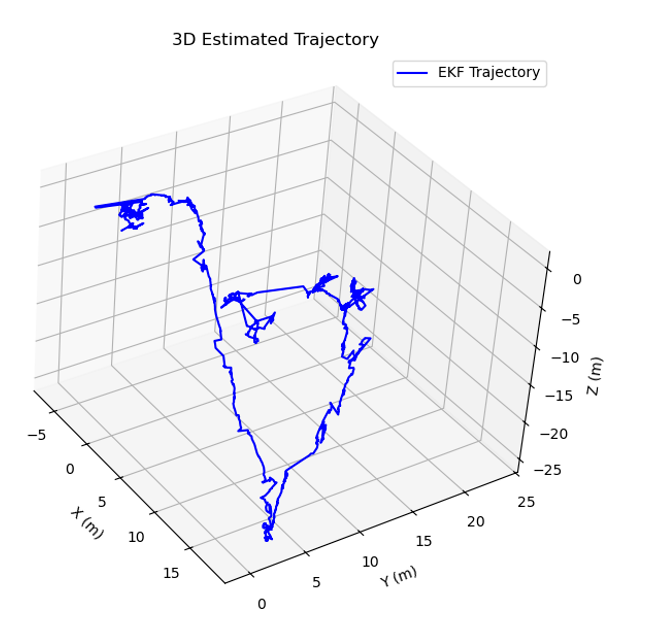
\includegraphics[width=0.6\textwidth]{figures/ekf_R1e-4_Q1e-8.png}
  \caption{EKF trajectory, $R_{\text{cov}}=10^{-4}I$, $Q_{\text{cov}}=10^{-8}I$.}
\end{figure}

\textbf{*NOTE} (from the original report): the world frame was taken to be the system's initial pose.
The issue is that gravity was subtracted assuming the world frame's $z$ axis is exactly vertical at
time 0, but we did not know for certain whether it actually is. The results along the $z$ axis should
therefore be interpreted with this in mind.

\subsection*{Discussion (added)}
The qualitative difference between the three runs is consistent with what the Kalman-gain equation
predicts: lowering $R$ relative to $Q$ makes the filter trust the IMU-driven prediction more, so the
corrections from VO are down-weighted and the trajectory follows the (drift-prone, double-integrated)
inertial model more closely; lowering $Q$ relative to $R$ does the opposite, pulling the trajectory
toward the VO-only estimate shown in Figs.~5--6, which does not drift in the same way but is noisier
frame-to-frame. The balanced setting (Sec.~4.1) sits between the two, which is the qualitative
behavior one would want from the fusion, even though — per the implementation note in Sec.~3.1 — the
specific numerical values of $R$ and $Q$ used here are fixed constants chosen by hand rather than the
physically-derived or per-step values computed elsewhere in the pipeline.

\section*{Limitations and possible improvements (added)}
\begin{itemize}[leftmargin=*]
  \item \textbf{Constant, hand-tuned $R$ and $Q$.} As noted in Secs.~2.6 and 3.1, both the
  noise-density-derived $R_{\text{cov}}$ and the per-step VO covariance $Q_{\text{cov},k}$ are computed
  in the code but not actually used by the final EKF run, which instead uses fixed constants. Feeding
  both back in would let the filter adapt its trust in each branch automatically, frame by frame,
  instead of relying on a single global tuning choice.
  \item \textbf{No loop closure or global optimization.} The pipeline is a purely sequential, online-style
  filter (frame-to-frame fusion only); there is no mechanism to detect revisited places or to perform a
  global bundle adjustment, so errors accumulate monotonically over the trajectory, as is visible in the
  gap between the VO start and end points in Figs.~5--6.
  \item \textbf{Euler-angle orientation state.} Euler angles are simple to reason about but suffer from
  gimbal lock and are not the most numerically stable choice for orientation in a filter; a quaternion
  or Lie-algebra ($SO(3)$) parametrization is the more standard choice in modern VIO systems (e.g.
  MSCKF, VINS-Mono) and would avoid this issue, at the cost of a more involved Jacobian derivation.
  \item \textbf{Decoupled VO front end.} Visual odometry here is computed independently per frame pair
  (features $\to$ 3D points $\to$ Kabsch) and only afterward fed into the EKF as a black-box
  measurement; a tightly-coupled filter that reasons jointly over IMU and feature-reprojection residuals
  (as in MSCKF-style filters) typically makes better use of the same raw data.
\end{itemize}

\end{document}
